% !Mode:: "TeX:UTF-8"%確保文檔utf-8編碼
\documentclass[tikz,border=2pt]{standalone}
\usepackage{pgfplots}
\pgfplotsset{compat=newest}
\usetikzlibrary{patterns,calc}
\begin{document}
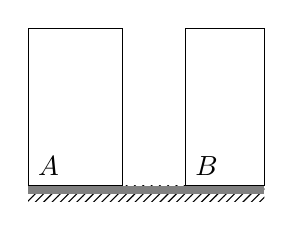
\begin{tikzpicture}
\draw (0,0) node[above right] {$A$} rectangle (1.2,2);

\draw (2,0) node[above right] {$B$} rectangle (3,2);


\begin{scope}
\fill[pattern = north east lines] (0,0) rectangle (3,-0.2);
\fill[color=black!50] (0,0) rectangle (3,-0.1);
\end{scope}



\end{tikzpicture}
\end{document}